\documentclass[12pt]{article}

%% bibliography stuff -- this needs come before the preamble inclusion
\usepackage[backend=bibtex,sorting=none]{biblatex}
\bibliography{\string~/Documents/academics/global_academics/global_bib.bib}
\usepackage{hyperref}

\def\gc{\overset{\text{GC}}{\rightarrow}}  % Granger causality arrow
\def\pwgc{\overset{\text{PW}}{\rightarrow}}  % Granger causality arrow
\def\te{\overset{\mathcal{T}}{\rightarrow}}  % Transfer entropy arrow
\def\gcg{\mathcal{G}}  % Granger-causality graph
\def\VAR{\mathsf{VAR}}  % VAR(p) model
\def\B{\mathsf{B}}  % Filter B
\def\wtB{\widetilde{\B}}  % General filter B
\def\A{\mathsf{A}}  % Filter A
\def\H{\mathcal{H}}  % Hilbert space

\newcommand{\linE}[2]{\hat{\E}[#1\ |\ #2]}  % Linear projection
\newcommand{\linEerr}[2]{\xi[#1\ |\ #2]}  % Error of linear projection
\newcommand{\pa}[1]{pa(#1)}  % Parents of a node
\newcommand{\anc}[1]{\mathcal{A}(#1)}  % Ancestors of a node
\newcommand{\ancn}[2]{\mathcal{A}_{#1}(#2)}  % nth ancestors of a node
\newcommand{\gpn}[2]{gp_{#1}(#2)}  % nth generation grandparents
\newcommand{\gcgpath}[4]{#1 \rightarrow #2_1 \rightarrow \cdots \rightarrow #2_{#3} \rightarrow #4}

% \usepackage{fullpage}
\usepackage{framed}

% Figures
\usepackage{graphicx}
\usepackage{caption}
% \usepackage{subcaption}
\usepackage{wrapfig}
\usepackage{svg}

% Math packages, theorem definitions and numbering
\usepackage{amsmath}
\usepackage{amssymb}
\usepackage{amsthm}
\usepackage{mathrsfs} % Fancy scripted font
\usepackage{bm}  % Bold math
\usepackage{centernot}  % \centernot\implies looks better

% Misc packages
\usepackage[linesnumbered, ruled, vlined]{algorithm2e}
% \usepackage{algorithm2e} %{algorithm} environment
\usepackage{soul}  % \hl highlighting
\usepackage{color}
\usepackage{mathtools}  % For my \ceil function

% Theorems (with italics)
\theoremstyle{plain}  % Style definition removes italics
\newtheorem{theorem}{Theorem}
\newtheorem{corollary}{Corollary}
\newtheorem{proposition}{Proposition}
\newtheorem{lemma}{Lemma}

\theoremstyle{definition}
\newtheorem{remark}{Remark}
\newtheorem{definition}{Definition}
\newtheorem{example}{Example}
\newtheorem{assumption}{Assumption}

% keywords
\providecommand{\keywords}[1]{\textbf{\textit{Keywords---}} #1}

% General
\def\defeq{\overset{\Delta}{=}}  % Equal with triangle
\def\cl{\mathsf{cl\ }}  % Closure
\newcommand{\sgn}[1]{\mathsf{sgn}(#1)}  % sign function

% Calculus
\def\d{\mathsf{d}}  % Differential operator

% Functions
\def\ln{\mathsf{ln\ }}  % Natural logarithm
\DeclarePairedDelimiter{\ceil}{\lceil}{\rceil}  % Ceiling

% Probability
\def\H{\mathcal{H}}  % Hilbert space
\def\E{\mathbb{E}}  % Expectation
\def\Var{\text{Var}}  % Variance
\def\P{\mathbb{P}}  % Probability Measure
\def\F{\mathcal{F}}  % A sigma algebra
\def\sX{\mathcal{X}}  % Another sigma algebra
\def\KL{\mathbf{D}_{KL}}  % KL divergence
\def\bF{\mathbf{F}}  % Whole F-meas space
\def\GP{\mathcal{GP}}  % Gaussian process

% Standard sets
\def\Z{\mathbb{Z}}  % Set of integers
\def\R{\mathbb{R}}  % Set of real numbers
\def\C{\mathbb{C}}  % Set of complex numbers
\def\N{\mathbb{N}}  % Set of natural numbers
\def\ball{\mathbb{B}}  % Open ball
\def\clball{\overline{\ball}}  % Closed ball

% Linear algebra
\def\rk{\mathsf{rk }}  % The rank
\def\tr{\mathsf{tr }}  % The trace
\def\T{\mathsf{T}}  % Transpose notation
\def\c{\mathsf{c}}  % complement
\def\dg{\mathsf{dg }}   %  Diagonal vector of a matrix
\def\Dg{\mathsf{Dg }}   %  Diagonal matrix from a vector
\def\ind{\mathbf{1}}  % Ones vector or indicator
\def\matvec{\textbf{vec}}  % Vector operator
\def\<{\langle}  % < Inner product
\def\>{\rangle}  % > Inner product
\newcommand{\inner}[2]{\langle #1, #2 \rangle}  % Inner product
\newcommand{\innerT}[2]{#1^\T #2}  % Inner product for finite vectors

% Convex analysis
\def\conv{\mathsf{conv }}  % Convex hull
\def\prox{\mathsf{prox }}  % Proximity operator

% -----------------
% The given symbol or text (\text{mytext}) in a circle
% To be used always in math mode
\newcommand{\circlesign}[1]{ 
    \mathbin{
        \mathchoice
        {\buildcirclesign{\displaystyle}{#1}}
        {\buildcirclesign{\textstyle}{#1}}
        {\buildcirclesign{\scriptstyle}{#1}}
        {\buildcirclesign{\scriptscriptstyle}{#1}}
    } 
}

\newcommand\buildcirclesign[2]{%
    \begin{tikzpicture}[baseline=(X.base), inner sep=0, outer sep=0]
    \node[draw,circle] (X)  {\ensuremath{#1 #2}};
    \end{tikzpicture}%
}
% -----------------


\graphicspath{{./figures/}}

\title{Structure Learning for $\VAR(p)$ Models}
\author{R. J. Kinnear, R. R. Mazumdar}

\begin{document}
\maketitle
\abstract{We study Granger Causality and propose a structure learning
  heuristic for uncovering a parsimonious representation of large
  $\mathsf{VAR}(p)$ models.}

\section{Introduction and Review}
\label{sec:introduction}
Consider a collection of stochastic processes producing observations
at discrete time intervals.  Are the underlying processes dependent?
Can we quantify any of the underlying relationships?  Can the arrow of
time help us to distinguish a directionality or flow of dependence
among our observed series?  In this paper we contribute to the
understanding of the notion of Granger-Causality
\cite{granger1969investigating} as a tool for answering these questions.

Though the notion of causality is a philosophically slippery concept,
it is fundamental to the way we understand the world and to the
progress of science in general.  Indeed, without faith in the
consistency of causal interactions the results of experimental science
could not be generalized or applied in any meaningful way.  In the
case of Granger-Causality, we state that if an event '$A$' provides us
with unique (that is, not available anywhere else) information about a
later event $B$, then $A$ must have a causal impact on $B$.  As
opposed to the notion of Causation promoted by Pearl
\cite{pearl2000art}, this is an entirely model-free notion of cause,
and instead leverages the intuition that a cause must precede it's
effect.

In practice, Granger's notion of causation it not a convincing test
for \textit{true} causation, since our statements about causation are
highly dependent upon the data that we are able to observe.  We prefer
instead to interpret Granger causality as a means of uncovering a flow
of ``information'' or ``energy'' through some underlying graph of
interactions.  Though this graph cannot be observed directly, we will
infer it's presence as a latent structure among our observed time
series data.

Finding the ``best'' graph structure consistent with observed data is
generally an extremely challenging problem, though the comparison of
quality between different structures, and hence the notion of
``best'', needs to be quantified.  In applications where we are
interested merely in minimizing the mean squared error of a linear
one-step-ahead predictor, then we will naturally desire an entirely
dense graph of connections, since each edge can only serve to reduce
estimation error.  However, since the number of edges scales
quadratically in $n$, it is imperative to infer a sparse causality
graph for large systems, both to avoid overfitting observed data, as
well as to aid the interpretability of the results.

In \cite{bach2004learning} the authors apply a local search heuristic
to an AIC penalized approximation of the likelihood where at each
iteration an edge is either added, removed, or reversed.  This is a
common approach to combinatorial optimization due to it's simplicity,
but is liable to get stuck in shallow local minima.

A second and wildly successful heuristic is the LASSO regularizer
\cite{tibshirani1996regression}, which can be understood as a natural
convex relaxation to penalizing the count of the non-zero edges.  The
LASSO enjoys strong theoretical guarantees \cite{wainwright2009sharp},
even in the case of time series data \cite{basu2015}
\cite{wong2016lasso}.

From a Bayesian perspective, spike-and-slab priors can be used to
estimate the probability of an edge's inclusion, after which a graph
can be chosen heuristically by thresholding or searching for the MAP
graph structure.

Our contribution is to provide an alternative heuristic based on
minimum spanning trees, inspired by our result in section
\ref{sec:theory} that the true causality graph can be recovered from
pairwise information alone in the case that the underlying graph is a
directed forest.  We compare this algorithm to a grouped LASSO
\cite{yuan2006model}, local search, and a Bayesian posterior
probability thresholding scheme.

%% -Can we also formulate an SDP relaxation?
%% -Fit trees jointly or via coordinate descent?

\section{Theory}
\label{sec:theory}
\subsection{Formal Setting}
Consider the space $L_2(\Omega)$, the usual Hilbert space of finite
variance random variables over a probability space
$(\Omega, \mathcal{F}, \mathbb{P})$ having inner product
$\inner{x}{y} = \E[xy]$.  We will denote the collection vectors of
such random elements as $L_2^n(\Omega)$ or simply $L_2^n$.

We will work with a discrete time and wide-sense stationary process
$x(t)$ taking elements in $L_2$.  We suppose that $x(t)$ has zero
mean, $\E x(t) = 0$, and the matrix valued covariance sequence
$R(\tau) \overset{\Delta}{=} \E x(t)x(t - \tau)^\T$ is absolutely summable and has a spectra $S(\omega)$:

\begin{equation}
  \label{eqn:fourier_pair}
  \begin{aligned}
    R(\tau) &= \frac{1}{2\pi}\int_{-\pi}^\pi S(\omega) e^{j\tau\omega}\d \omega,\\
    S(\omega) &= \sum_{\tau=-\infty}^\infty R(\tau)e^{-j\tau\omega}.
  \end{aligned}
\end{equation}

We will also work frequently with the spaces spanned by the values of
such a process

\begin{equation}
  \label{eq:hilbert_space_defn}
  \begin{aligned}
    \H^x &= \cl \{\sum_{\tau = -T}^T a_\tau^\T x(t - \tau)\ |\ a_\tau \in \R^n, T \in \N\} \subseteq L_2(\Omega),\\
    \H_t^x &= \cl \{\sum_{\tau = 0}^T a_\tau^\T x(t - \tau)\ |\ a_\tau \in \R^n, T \in \N\} \subseteq L_2(\Omega),
  \end{aligned}
\end{equation}

where the closure is naturally in mean-square.  $\H_t^x$ is the space
spanned by the values of $x(t)$ between the ``infinite past'' and
``now'', we will often omit the superscript $x$ which should be clear
from context.  Evidently these spaces are separable and as closed
subspaces of a Hilbert space they are themselves Hilbert.  We will
denote the spaces generated in analagous ways by particular components
of $x$ as e.g. $\H_t^{(i, j)}$, $\H_t^{i}$ or by all but particular
components as e.g. $\H_t^{-j}$.

As a consequence of the Wold decomposition theorem \cite{lindquist},
every such sequence has the ``moving average'' $MA(\infty)$
representation

\begin{equation}
\label{eqn:wold}
  x(t) = c(t) + \sum_{\tau = 0}^\infty A(\tau) w(t - \tau),
\end{equation}

where $c(t)$ is a perfectly predictable sequence\footnote{$c(t)$ is
  perfectly predictable if any sample $c(t_0)$ is enough to determine
  $c(t)$ for every $t$.  For example,
  $c(t) = \text{sin}(2\pi t + \Theta);\; \Theta \sim \mathcal{U}[-\pi,
  \pi]$}, and $w(t)$ is an uncorrelated sequence having a diagonal
covariance and $A(0) = I$.  We will assume that $c(t) = 0$, which in
practice is to say that it has been accurately estimated and removed.

Furthermore, we assume that the spectra is uniformly bounded away from
$0$:
$\exists \delta:\ \delta I \preceq S(\omega) \preceq \frac{1}{\delta}
I\ \forall \omega$ so that the Wold representation can be inverted to
yield the $VAR(\infty)$ form

\begin{equation}
  \label{eqn:ar_representation}
  x(t) = \sum_{\tau = 1}^\infty B(\tau) x(t - \tau) + v(t),
\end{equation}

where $v(t)$ is an uncorrelated sequence with covariance $\Sigma_v$.

The equations (\ref{eqn:wold}), (\ref{eqn:ar_representation}) can be
represented as $x(t) = \A(z)w(t) = \B(z)x(t) + v(t)$ via the action of
the operators (LTI filters)
$\A(z) \defeq \sum_{\tau = 0}^\infty A(\tau)z^{-\tau}$ and
$\B(z) \defeq \sum_{\tau = 1}^\infty B(\tau)z^{-\tau}$ where the
operator $z^{-1}$ is the backshift operator acting on $\H$.  Since
$||z^{-1}|| = 1$, the inversion formulae

\begin{equation}
  \label{eqn:lsi_inversion}
  \A(z) = (I - \B(z))^{-1} = \sum_{k = 0}^\infty \B(z)^k
\end{equation}

are valid.
\subsection{Granger Causality}

\begin{definition}[Granger Causality]
  For the WSS series $x(t)$ we say that component $x_j$
  \textit{Granger-Causes} (GC) component $x_i$ (with respect to $x$)
  and write $x_j \gc x_i$ if given Hilbert spaces
  $\H_{t - 1}$, $\H^{-j}_{t - 1}$

\begin{equation}
  \linEerr{x_i(t)}{\H_{t - 1}} < \linEerr{x_i(t)}{\H^{-j}_{t - 1}},
\end{equation}

where $\xi[x \ |\ \H] = \E (x - \linE{x}{\H})^2$ is the mean squared
estimation error and $\linE{x}{\H} = \text{proj}_{\H}(x)$ denotes the
(unique) projection onto the Hilbert space $\H$.
\end{definition}

This notion captures the idea that the process $x_j$ provides
information about $x_i$ that is not available from elsewhere.  The
caveat ``with respect to $x$'' is important in that GC relations can
change when components are added to or removed from our collection $x$
of observations, e.g. new GC relations can arise if we remove the
observations of a common cause, and existing GC relations can
disappear if we observe a new mediating series.

The notion is closely related to the information theoretic measure of
transfer entropy, indeed, if everything is Gaussian then they are
equivalent \cite{barnett2009granger}.

\begin{theorem}[Granger Causality Equivalences]
  \label{thm:granger_causality_equivalences}
  Let $x(t)$ be a WSS process with absolutely summable covariance
  sequence, and spectral density uniformly bounded above and below.  Denote by
  $\xi_{ij} \defeq \linEerr{x_i(t)}{\H^{-j}}$ and
  $\xi_i \defeq \linEerr{x_i(t)}{\H_t}$.  Then, the following are equivalent:

  \begin{enumerate}
    \item{$x_j \not\gc x_i$}
    \item{$\forall \tau \in \N_+\ B_{ij}(\tau) = 0$}
    \item{$\mathcal{F}_{j \rightarrow i} \defeq \ln\frac{\xi_i}{\xi_{ij}} = 0$}
    \item{$\H_t^{i} \perp \H_{t - 1}^{j}\ |\ \H_{t - 1}^{-j}$}
    \item{$\linE{x_i(t)}{\H_{t - 1}^{-j}} = \linE{x_i(t)}{\H_{t - 1}}$}
    % \item{\hl{Wold $A(\tau)$ condition}}
    % \item{Tie in the 0s of $S(\omega)^{-1}$, though this isn't immediately directed.}
  \end{enumerate}
\end{theorem}

Statement (4) means that
$(y - \linE{y}{\H_{t - 1}^{-j}}) \perp (z - \linE{z}{\H_{t -
    1}^{-j}})\ \forall y \in \H_t^i,\ z \in \H_{t - 1}^j$, which is an
appealing geometric statement that there is no direct feedback from
$x_j$ to $x_i$ \cite{lindquist}.

\begin{proof}
  The equivalence $(1) \iff (3)$ is essentially a restatement of the
  definition, but is in line with the seminal work of Geweke
  \cite{geweke1982measurement}, \cite{geweke1984}.

  The equivalence $(3) \iff (5)$ is also immediate from the
  definitions i.e. the projections are equal if and only if the errors
  are equal.

  $(1) \implies (2)$: The projection for $x_i(t)$ onto $\H_{t - 1}$ is
  (by definition) given by a form similar to equation
  \ref{eqn:ar_representation}:

\[
  \E|x_i(t) - \linE{x_i(t)}{\H_{t - 1}}|^2 = \E|v_i(t) + \sum_{\tau = 1}^\infty \sum_{k = 1}^n (B_{i, k}(\tau) - \hat{B}_{i, k}(\tau))x_k(t - \tau)|^2.
\]

Since $v(t)$ in equation \ref{eqn:ar_representation} is temporally
uncorrelated, it follows that the optimal projection is given by the
model coefficients themselves.  This holds similarly for the
projection onto $\H_{t - 1}^{-j}$.  Then by $(1)$ we have

\[
  \E|x_i(t) - \sum_{\tau = 1}^\infty \sum_{k = 1}^n B_{i, k}(\tau)x_k(t - \tau)|^2 = \E|x_i(t) - \sum_{\tau = 1}^\infty\sum_{k \ne j}B_{i, k}(\tau)x_k(t - \tau)|^2
\]

By the uniqueness of the projection we must have
$\forall \tau\ B_{i, j}(\tau) = 0$.

$(2) \implies (4)$: In computing $(y - \linE{y}{\H_{t = 1}^{-j}})$ for
$y \in \H_t^i$ it is sufficient to consider $y = x_i(t)$ since
$\H_{t - 1}^i \subseteq \H_{t - 1}^{-j}$, in which case
$(x_i(t) - \linE{x_i(t)}{\H_{t = 1}^{-j}}) = v_i(t)$.  $(4)$ follows
since $v_i(t) \perp \H_{t - 1}$ and
$\forall z \in \H_{t - 1}^j\ (z - \linE{z}{\H_{t - 1}^{-j}}) \in \H_{t
  - 1}$

\hl{TODO: $(4) \implies (1)$}
  
\end{proof}

% The following propositions justify various modifications of $x(t)$
% applied in practice to massage $x(t)$ into a form amenable to more
% standard tools.

% \begin{theorem}[General Invariance]
%   \hl{Under what conditions is this actually true?}

%   Let $\zeta(t)$ be a stationary discrete time stochastic process.  Let
%   $F, G$ be (possibly nonlinear and time varying) invertible filtering
%   operations and $f(t)$, $g(t)$ be perfectly predictable and such that
%   $x_j(t) \defeq F(\zeta_j - f)(t), x_i(t) \defeq G(\zeta_i - g)(t)$ are W.S.S.  Then,

% \begin{equation}
%     x_j \gc x_i \iff \zeta_j \te \zeta_i
%   \end{equation}
% \end{theorem}

\begin{proposition}[Invariance Under Invertible and Deterministic Modifications]
  Let $x(t)$ be a WSS process with absolutely summable covariance
  sequence, and spectral density uniformly bounded above and below.  Let
  $F(z), G$ represent univariate and invertible
  linear-time-invariant filters.  And, let $f(t), g(t)$ be perfectly
  predictable processes.  Then,

  \begin{equation}
    x_j \gc x_i \iff F(x_j - f)(t) \gc G(x_i - g)(t)
  \end{equation}

\begin{proof}
  \hl{TODO}
\end{proof}
\end{proposition}

\subsection{Pairwise Granger Causality}
\label{sec:pwgc}
Recall that Granger-causality in general must be understood with
respect to a particular universe of observations.  If $x_j \gc x_i$
with respect to $x_{-k}$, it may not hold with respect to $x$.  For
example, $x_k$ may be a common ancestor which when observed completely
explains the connection from $x_j$ to $x_i$.  In particular, we will
study \textit{pairwise} Granger-causality.

\begin{definition}[Pairwise Granger-causality]
  We will say that $x_j$ pairwise Granger-causes $x_i$ and write
  $x_j \pwgc x_i$ if $x_i$ Granger-causes $x_j$ with respect only to
  $(x_i, x_j)$.
\end{definition}

This notion is of interest for a variety of reasons.  From a purely
theoretical or conceptual standpoint, we will seek to understand when
and how pairwise causality can capture the idea of ``flow of
information'' in the underlying graph.  It will also be useful to
reason about what the conditions under which \textit{unobserved}
components of $x(t)$ may or may not interfere with inference in the
actually observed components.  Finally, we will seek to construct
practical estimation procedures based purely on pairwise causality
tests and understand their properties.

We first need to establish some graph theoretic notation and
terminology, collected formally in definitions for the reader's
convenient reference.

\begin{definition}[Causality graph, Parents]

Remaining in the context of a collection of $n$ WSS processes
$x(t) = \big(x_1(t), \ldots, x_n(t)\big)$, we define the Granger-causality
graph $\gcg$ to be the directed graph formed on $n$ vertices where an
edge $(j, i) \in \gcg$ if and only if $x_j \gc x_i$.

We refer to the set of \textit{parents} of $x_i$ in $\gcg$ by
$\pa{i}$, that is, $j \in \pa{i} \iff x_j \gc x_i$.
\end{definition}

\begin{definition}[Grandparents, ancestors]
The set of level $\ell$ \textit{grandparents} of node $i$, denoted
$\gpn{\ell}{i}$, is the set such that $j \in \gpn{\ell}{i}$ if and only if
there is a \textit{directed and cycle-free path} of length $\ell$ in
$\gcg$ from $j$ to $i$ \textit{or} if $j = i$ and there is a cycle of
length $\ell$ starting at $i$ and ending back at $i$, that is, $i$ can be
it's own grandparent.  Clearly, $\pa{i} = \gpn{1}{i}$.

Finally, the set of \textit{level $\ell$ ancestors} of
$i$: $\ancn{\ell}{i} = \bigcup_{\lambda \le \ell}\gpn{\lambda}{i}$ is the set such that
$j \in \ancn{\ell}{i}$ if and only if there is a directed and cycle-free
path of length $\ell$ \textit{or less} in $\gcg$ from $j$ to $i$
\textit{or} if $j = i$ and there is a directed cycle of length $\ell$ or
less from $i$ back to $i$ in $\gcg$.  The set of \textit{all
  ancestors} of $i$ (i.e. $\ancn{n}{i}$) is denoted simply $\anc{i}$.
\end{definition}

Even though the definitions of Granger-causality naturally suggests
that each node in the graph should have a self-loop (unless the node
is simply independent noise) we will not include nodes in their own
parent sets: $i \not\in \pa{i} \subseteq \anc{i}$.  However, we do not
immediately assume that $\gcg$ is a DAG, and so \textit{we will allow for $i$
to be it's own ancestor}.

The edges of the Granger-causality graph $\gcg$ can be given a general
notion of ``weight'' by associating an edge $(j, i)$ with a
\textit{strictly causal} LTI filter

\begin{equation}
  \label{eqn:filter}
  \B_{ij}(z) = \sum_{\tau = 1}^{\infty} B_{ij}(\tau)z^{-\tau}
\end{equation}

from the $\VAR$ representation of equation
\ref{eqn:ar_representation}.  We will represent the action
(convolution) of this filter compactly by taking $z^{-1}$ as the
backshift operator on $\ell_2^n(\Omega, \mathcal{F}, \mathbb{P})$ when
convenient

\begin{equation}
  \sum_{\tau = 1}^\infty B_{ij}(\tau)x_j(t - \tau) \defeq \B_{ij}(z)x_j(t).
\end{equation}

% What if we take this as the definition of PWGC?  then, in a simply causal graph
% the "normal" definition becomes a theorem.  Or, if lem:pwgc_anc is true then
% maybe that is good enough?

From the $\VAR$ representation of $x(t)$ there is clearly a tight
relationship between each node and it's parent nodes, indeed

\begin{equation}
  \label{eqn:parent_expansion}
  x_i(t) = v_i(t) + \B_{ii}(z)x_i(t) + \sum_{k \in \pa{i}}\B_{ik}(z)x_k(t).
\end{equation}

% When is this guaranteed w.r.t. the full system?
Furthermore, if the filter $\B_{ii}$ is invertible, we can write

\begin{equation*}
  \begin{aligned}
    (1 - \B_{ii}(z))x_i(t) &= v_i(t) + \sum_{k \in \pa{i}}\B_{ik}(z)x_k(t)\\
    \implies x_i(t) &= (1 - \B_{ii}(z))^{-1}\big[v_i(t) + \sum_{k \in \pa{i}}\B_{ik}(z)x_k(t)\big]\\
    &= \wtB_{ii}(z)v_i(t) + \sum_{k \in \pa{i}}\wtB_{ik}(z)x_k(t)
  \end{aligned}
\end{equation*}

% In general, we will write $\wtB$ for arbitrary filters maintaining the
% convention that $\wtB_{ii}$ is a filter that modifies the future of
% $x_i$ from it's past and $\wtB_{ij}$ a filter modifying $x_i$ from the
% past of $x_j$.  We will use the convention that the filter
% $\widetilde{\B}$ will represent simply ``a filter'' and is not
% necessarily the same as the filters serving as edge weights in $\gcg$
% (indeed, $\wtB$ will often be $0$), and moreover, we will allow for
% $\widetilde{\B}$ to potentially change from place to place and even
% from line to line in the same sequence of calculations as it's exact
% properties or specification are not important.

We continue to develop the relationship between $x_i$ and it's family tree.

\begin{proposition}[Ancestor Expansion]
  \label{prop:parent_expanding}
  The component $x_i(t)$ of $x(t)$ can be represented as a sum of
  linear filtering operations acting on the driving noise $v_i$ of
  $x_i$ as well as the parents of $x_i$:

  \begin{equation}
    x_i(t) = \wtB_{ii}(z)v_i(t) + \sum_{k \in \pa{i}}\wtB_{ik}(z)x_k(t).
  \end{equation}

  Moreover, $x_i$ can be expanded in terms of it's ancestors and
  driving noise only:

  \begin{equation}
    \label{eqn:ancestor_expansion}
    x_i(t) = \A_{ii}(z)v_i(t) + \sum_{k \in \anc{i} \setminus\{i\}}\A_{ik}(z)v_k(t),
  \end{equation}

  where $\A(z) = \sum_{\tau = 0}^\infty A(\tau)$ is the filter from
  the Wold decomposition representation of $x(t)$, equation
  (\ref{eqn:wold}).
\end{proposition}

This statement is ultimately about the sparsity pattern in the Wold
decomposition matrices $A(\tau)$ since
$x_i(t) = \sum_{\tau = 0}^\infty \sum_{j = 1}^n a_{ij}(\tau)v_j(t -
\tau)$.  The proposition states that $\A_{ij}(\tau) = 0$ unless
$j \in \anc{i}$.

% \begin{proof}
%   The formula (\ref{eqn:parent_expansion}) was established in the
%   preceding paragraph and serves as a starting point for the induction
%   hypothesis:

%   \begin{equation}
%     \label{eqn:induction}
%     x_i(t) = \wtB_{ii}(z)v_i(t) + \sum_{k \in \ancn{\ell - 1}{i}\setminus \{i\}}\wtB_{ik}(z)v_k(t) + \sum_{k \in \gpn{\ell}{i} \setminus \{i\}}\wtB_{ik}(z)x_k(t).
%   \end{equation}

%   The base case follows by expanding each $x_k$ in equation \ref{eqn:induction} via equation \ref{eqn:parent_expansion}, but we skip the calculations since they are nearly identical to the following induction step:

%   \begin{align*}
%     x_i(t) &= \wtB_{ii}(z)v_i(t) + \sum_{k \in \ancn{\ell - 1}{i}\setminus \{i\}}\wtB_{ik}(z)v_k(t) + \sum_{k \in \gpn{\ell}{i} \setminus \{i\}}\wtB_{ik}(z)x_k(t)\\
%            &\overset{(a)}{=} \wtB_{ii}(z)v_i(t) + \sum_{k \in \ancn{\ell - 1}{i}\setminus \{i\}}\wtB_{ik}(z)v_k(t) + \sum_{k \in \gpn{\ell}{i} \setminus \{i\}}\wtB_{ik}(z)\big[\wtB_{kk}v_k(t)\\
%     &\ \ \ \  + \wtB_{ki}(z)x_i(t) + \sum_{h \in \pa{k}\setminus \{i\}}\wtB_{kh}(z)x_h(t)\big]\\
%     &\overset{(b)}{=} \wtB_{ii}(z)v_i(t) + \sum_{k \in \ancn{\ell}{i} \setminus \{i\}}\wtB_{ik}(z)v_k(t) + \sum_{k \in \gpn{\ell + 1}{i} \setminus \{i\}}\wtB_{ik}(z)x_k(t).
%   \end{align*}

%   Where equality $(a)$ follows by expanding each $x_k$ with equation \ref{eqn:parent_expansion} and $(b)$ requires the inversion of $\big(1 - \sum_{k \in \gpn{\ell}{i}\setminus\{i\}}\wtB_{ik}(z)\wtB_{ki}(z)\big)$ as well as using the fact that $\ancn{\ell}{i} = \ancn{\ell - 1}{i}\cup\gpn{\ell}{i}$.  We here remind the reader of our earlier established convention that $\wtB$ simply represents the existence of a filter (possibly 0) and can change from place to place.

% The induction terminates after $n$ steps since in a graph with $n$ nodes $\gpn{n + 1}{i} = \emptyset$

% % Where step $(a)$ requires the inversion of $1 - \sum_{k \in \pa{i}}\wtB_{ik}(z)\wtB_{ki}(z)$.

% %   \begin{align*}
% %     x_i(t) &= \wtB_{ii}(z)v_i(t) + \sum_{k \in \pa{i}}\wtB_{ik}(z)x_k(t)\\
% %            &= \wtB_{ii}(z)v_i(t) + \sum_{k \in \pa{i}}\wtB_{ik}(z)\big[\wtB_{kk}v_{k}(t) + \wtB_{ki}(z)x_i(t) + \sum_{h \in \pa{k}\setminus \{i\}}\wtB_{kh}(z)x_h(t) \big]\\
% %            &\overset{(a)}{=} \wtB_{ii}(z)v_i(t) + \sum_{k \in \pa{i}}\wtB_{ik}(z)v_{k}(t) + \sum_{k \in \gpn{2}{i} \setminus \{i\}}\wtB_{ik}(z)x_k(t)
% %   \end{align*}

% % Where step $(a)$ requires the inversion of $1 - \sum_{k \in \pa{i}}\wtB_{ik}(z)\wtB_{ki}(z)$.

% \end{proof}
% \textbf{this is an alternative proof, I think superior to the one above}.

The matrix $\B(z)$ is analagous to a \textit{weighted adjacency
  matrix} for the graph $\gcg$.  And, in the same way that the
$k^{\text{th}}$ power of an adjacency matrix counts the number of
paths of length $k$ between nodes, $(\B(z)^k)_{ij}$ is a filter
isolating the ``action'' of $j$ on $i$ at a time lag of $k$ steps.
Though we only need the sparsity pattern of $\B(z)^k$ for the proof.

We state the following well known theorem as a lemma, proof follows
easily by induction.

\begin{lemma}
  \label{lem:adj_matrix}
  Let $S$ be the transposed adjacency matrix of the Granger-causality
  graph $\gcg$.  Then, $(S^k)_{ij}$ is the number of paths of length
  $k$ from node $j$ to node $i$.  Evidently, if
  $\forall k \in \N,\ (S^k)_{ij} = 0$ then $j \not\in \anc{i}$.
\end{lemma}

We now prove the proposition.

\begin{proof}
  From equation (\ref{eqn:ar_representation}), which we are assuming
  throughout the paper to be invertible, we can write

  \begin{equation*}
    x(t) = (I - \B(z))^{-1} v(t),
  \end{equation*}

  where $(I - \B(z))^{-1} = \A(z)$ due to the uniqueness of
  (\ref{eqn:wold}).  Since $\B(z)$ is stable, that is
  $|\lambda_{\text{max}}(B(z))| < 1$, for every $|z| \le 1$ we have

  \begin{equation}
    \label{eqn:resolvant_inv}
    (I - \B(z))^{-1} = \sum_{k = 0}^\infty \B(z)^k.
  \end{equation}

  Now, let $S$ be a $0-1$ matrix containing the sparsity pattern of
  $\B(z)$.  Then from lemma \ref{lem:adj_matrix} $S$ is the transpose
  of the adjacency matrix for $\gcg$ and hence $(S^k)_{ij}$ is
  non-zero if and only if $j \in \gpn{k}{i}$, and therefore
  $\B(z)^k_{ij} = 0$ if $j \not \in \gpn{k}{i}$.  The Cayley-Hamilton
  theorem can then be applied to represent the infinite sum of equation
  (\ref{eqn:resolvant_inv}) in terms only of \textit{finite} powers of
  $\B(z)$, so the application of lemma \ref{lem:adj_matrix} in the
  limit is not necessary.  Finally, since $\anc{i} = \cup_{k = 1}^n\gpn{k}{i}$
  we see that $\A(z)_{ij}$ is zero if $j \not\in \anc{i}$.

  Thence

  \begin{align*}
    x_i(t) &= (I - \B(z))^{-1}\\
    &= \sum_{j = 1}^n \A_{ij}(z) v_j(t)\\
    &= \A_{ii}(z) v_i(t) + \sum_{j \in \anc{i} \setminus \{i\}} \A_{ij}(z) v_j(t)\\
  \end{align*}
\end{proof}

Before moving onto our next proposition, we need two lemmas formalizing
some intuitively apparent facts.

\begin{lemma}
  \label{lem:subspace_sum_projection}
  Let $x \in \H$ where $\H$ is a Hilbert space having inner product $\inner{\cdot}{\cdot}$ and let $\{\H_n\}_{n = 0}^\infty$ be a collection of subspaces of $\H$ such that $x \perp \H_0$.  Then

  \begin{equation*}
    \linE{x}{\bigvee_{n = 0}^\infty\H_n} = \linE{x}{\bigvee_{n = 1}^\infty\H_n},
  \end{equation*}

  where $\H_2 \vee \H_2 = \cl \{\alpha + \beta\ |\ \alpha \in \H_1, \beta \in \H_2 \}$ is the closed sum of subspaces.
\end{lemma}
\begin{proof}
  We can apply the Gram-schmidt process to the collection of subspaces to obtain a sequence of orthogonal subspaces $\widetilde{\H}_0, \widetilde{\H}_1, \ldots$ with $\widetilde{\H}_0 = \H_0$, $\widetilde{\H}_n \subseteq \H_n$, and $\bigvee_{n = 0}^\infty\H_n = \bigoplus_{n = 0}^\infty \widetilde{\H}_n$, where $\oplus$ indicates the orthogonal sum of subspaces (which is always closed).  Then, we have an explicit representation of the projection

  \begin{align*}
    \linE{x}{\bigvee_{n = 0}^\infty\H_n} &= \sum_{n = 0}^\infty \inner{x}{x_n} x_n\\
    &\overset{(a)}{=} \sum_{n = 1}^\infty \inner{x}{x_n} x_n,
  \end{align*}

  where $x_n \in \widetilde{\H}_n \subseteq \H_n$ and $(a)$ follows because of our assumption that $x \perp \H_0$.  This establishes that the projection is infact a member of the smaller subspace $\bigvee_{n = 1}^\infty\H_n$, and since the error can only increase by projecting onto this smaller subspace, we have the conclusion.
\end{proof}

The following lemma is reproduced from \cite{lindquist} here for convenience.

\begin{lemma}[\cite{lindquist}]
  \label{lem:conditional_orthogonality_equivalence}
  Consider three closed subspaces of a Hilbert space $\mathcal{A}$, $\mathcal{B}$, $\mathcal{X}$.  The following statements are equivalent

  \begin{enumerate}
    \item{$\mathcal{A} \perp \mathcal{B}\ |\ \mathcal{X}$}
    \item{$\linE{\beta}{\mathcal{A} \vee \mathcal{X}} = \linE{\beta}{\mathcal{X}}\ \forall \beta \in \mathcal{B}$}
    % \item{$\linE{\beta}{\mathcal{A}} = \linE{\linE{\beta}{\mathcal{X}}}{\mathcal{A}}\ \forall \beta \in \mathcal{B}}$}
  \end{enumerate}
\end{lemma}
\begin{proof}
  Proceding from the definition of conditional orthogonality we have

  \begin{align*}
    &\inner{\alpha - \linE{\alpha}{\mathcal{X}}}{\beta - \linE{\beta}{\mathcal{X}}} = 0 \ \forall \alpha \in \mathcal{A}\ \beta \in \mathcal{B}\\
    &{\iff} \inner{\alpha + x - \linE{\alpha + x}{\mathcal{X}}}{\beta - \linE{\beta}{\mathcal{X}}} = 0 \ \forall \alpha \in \mathcal{A}\ \beta \in \mathcal{B}, x \in \mathcal{X}\\
    &\overset{(a)}{\iff} \inner{\alpha + x}{\beta - \linE{\beta}{\mathcal{X}}} = 0 \ \forall \alpha \in \mathcal{A}\ \beta \in \mathcal{B}, x \in \mathcal{X}\\
    &\overset{(b)}{\iff} \linE{\beta - \linE{\beta}{\mathcal{X}}}{\mathcal{A} \vee \mathcal{X}} = 0\ \forall \beta \in \mathcal{B}\\
    &\overset{(c)}{\iff} \linE{\beta}{\mathcal{A} \vee \mathcal{X}} = \linE{\beta}{\mathcal{X}},
  \end{align*}

  where $(a)$ follows since $(\beta - \linE{\beta}{\mathcal{X}}) \perp \mathcal{X}$ and $\linE{\alpha + x}{\mathcal{X}} \in \mathcal{X}$, $(b)$ since $z \perp \mathcal{X} \vee \mathcal{A} \iff \linE{z}{\mathcal{X} \vee \mathcal{A}} = 0$, and $(d)$ since $\linE{z}{\H_2} = \linE{\linE{z}{\H_2}}{\H_1}$ for $\H_2 \subseteq \H_1$.
  
  % This is property (vi) in Lindquist
  % \begin{align*}
  %   \langle \alpha - \linE{\alpha}{\mathcal{X}}, \beta - \linE{\beta}{\mathcal{X}} \rangle &= 0 \ \forall \alpha \in \mathcal{A}\ \beta \in \mathcal{B}\\
  %   \overset{(a)}{\iff} \langle \alpha, \beta - \linE{\beta}{\mathcal{X}} \rangle &= 0\ \forall \alpha \in \mathcal{A}\ \beta \in \mathcal{B}\\
  %   \overset{(b)}{\iff} \linE{\beta - \linE{\beta}{\mathcal{X}}}{\mathcal{A}} &= 0\ \forall \beta \in \mathcal{B}
  % \end{align*}

  % where $(a)$ follows because $\linE{\alpha}{\mathcal{X}} \in \mathcal{X}$ and $\beta - \linE{\beta}{\mathcal{X}} \in \mathcal{X}$, and $(b)$ follows since $\beta \perp \mathcal{A} \iff \linE{\beta}{\mathcal{A}} = 0$.
\end{proof}

\begin{proposition}
  \label{prop:ancestor_properties}
\hl{Need to refine this to exclude $k \rightarrow i \rightarrow j$ from 2.}

  In a Granger-causality graph $\gcg$, if $j \pwgc i$ then at least
  one of the following must hold

  \begin{enumerate}
    \item{$j \in \anc{i}$}
    \item{$\anc{i} \cap \anc{j} \ne \emptyset$}
  \end{enumerate}
\end{proposition}
\begin{proof}
  We will show the contrapositive.  Assume that $j \not \in \anc{i}$ and $\anc{i} \cap \anc{j} = \emptyset$, then $\forall \tau \in \Z_+,\ \E x_i(t)x_j(t - \tau) = 0$ since from the representation (\ref{eqn:parent_expansion}) we have

  \begin{align*}
    \E x_i(t)x_j(t - \tau) &= \E \big(\A_{ii}(z)v_i(t)\big)\big(\A_{jj}(z)v_j(t - \tau)\big)\\
    &+ \sum_{k \in \anc{i}}\E[\big(\A_{ik}(z)v_k(t)\big)v_j(t - \tau)] + \sum_{k \in \anc{j}}\E[v_i(t) \big(\A_{jk}(z) v_k(t - \tau)\big)]\\
    &+ \sum_{k \in \anc{i} \setminus i}\sum_{\ell \in \anc{j} \setminus j}\E[\big(\A_{ik}(z)v_k(t)\big)\big(\A_{j\ell}(z)v_\ell(t - \tau)\big)]\\
  \end{align*}

  Keeping in mind that $v(t)$ is an isotropic and uncorrelated sequence (i.e. $\forall \tau \in \Z,\ k \ne \ell \implies \E v_k(t)v_\ell(t - \tau) = 0$ and $\forall \tau \in \Z\setminus\{0\}\ \E v_i(t)v_i(t - \tau) = 0$), we will see that each of these above four terms are 0.  The first term since $i \pwgc i$ is not possible and hence the case $j = i$ is vacuous.  The second term is 0 since $j \not\in \anc{i}$.  The fourth term above is 0 since $\anc{i} \cap \anc{j} = \emptyset$.  For the third term, it is possible that (due to cycles) $i \in \anc{j}$ which requires more care, however similarly as before we can at least see that

  \begin{equation*}
    \sum_{k \in \anc{j}}\E[v_i(t) \big(\A_{jk}(z) v_k(t - \tau)\big)] = \E[v_i(t)\big(\A_{ji}(z)v_i(t - \tau)\big)].
  \end{equation*}

  However, $k \ne \ell \implies \A_{k\ell}(z) = 0$ (i.e. $\A(z) = I + A(1)z^{-1} + \cdots$) so $\A_{ji}(z)v_i(t - \tau)$ is strictly earlier in time, for $\tau \ge 0$, than $v_i(t)$ and hence $\E[v_i(t)\big(\A_{ji}(z)v_i(t - \tau)\big)] = 0$.  This establishes the fact that $H_t^{(i)} \perp \H_t^{(j)}$ where $H_t^{(i)} = \{\alpha x_i(t)\ |\ \alpha \in \R\}$ is the Hilbert space generated by the current sample of $x_i$.  It is clear that $\H_t^{(i)} = \bigvee_{\tau = 0}^\infty H_{t - \tau}^{(i)}$.

  \hl{TODO: Separate $H_t^i \perp \H_t^j \implies \H_t^i \perp \H_{t - 1}^j\ |\ \H_{t - 1}^i$ into a lemma and consolidate it with lemma 2, 3.}

  Then for every $s \ge 0$

  \begin{align*}
    \linE{x_j(t - s)}{\H_t^{(i)}} &= \linE{x_j(t - s)}{\bigvee_{\tau = 0}^\infty H_{t - \tau}^{(i)}}\\
    &\overset{(a)}{=} \linE{x_j(t - s)}{\bigvee_{\tau = 1}^\infty H_{t - \tau}^{(i)}}\\
    &= \linE{x_j(t - s)}{\H_{t - 1}^{(i)}},
  \end{align*}

  where $(a)$ follows from lemma (\ref{lem:subspace_sum_projection}).  Lemma (\ref{lem:conditional_orthogonality_equivalence}) tells us that this is equivalent to

  \begin{equation*}
    \H_t^{(i)} \perp \H_{t - 1}^{(j)}\ |\ \H_{t - 1}^{(i)},
  \end{equation*}

  so by theorem (\ref{thm:granger_causality_equivalences}) we conclude $j \not\pwgc i$.
\end{proof}

We can state some interesting corollaries of this result.

\begin{corollary}
  If the graph $\gcg$ is acyclic and if $j \pwgc i$ and $i \pwgc j$ then $\anc{i} \cap \anc{j} \ne \emptyset$.
\end{corollary}

It seems intuitive that a converse of \ref{prop:ancestor_properties}
would hold, i.e. $j \in \anc{i} \implies j \pwgc i$.  Unfortunately,
this is not the case in general, as different paths through $\gcg$ can
lead to cancellation.

\begin{example}
  \label{ex:diamond_cancellation}
  Firstly, on $n = 4$ nodes, ``diamond'' shapes can lead to cancellation on paths of length 2:

\begin{equation*}
  x(t) =
  \left[
    \begin{array}{cccc}
      0 & 0 & 0 & 0\\
      a & 0 & 0 & 0\\
      -a & 0 & 0 & 0\\
      0 & 1 & 1 & 0\\
    \end{array}
  \right] x(t - 1) + v(t),
\end{equation*}

with $\E v(t) = 0,\ \E v(t)v(t - \tau)^\T = \delta_\tau I$.

By directly calculating

\begin{align*}
  x_4(t) &= x_2(t - 1) + x_3(t - 1) + v_4(t)\\
         &= ax_1(t - 2) + av_2(t - 1) - ax_1(t - 2) -av_3(t - 1) + v_4(t)\\
         &= a(v_2(t - 1) - v_3(t - 1)) + v_4(t),
\end{align*}

we see that, since $v(t)$ is isotropic white noise, $1 \not\pwgc 4$.  The problem here is that there are multiple paths from $x_1$ to $x_4$.
\end{example}

\begin{figure}
  \centering
  \begin{subfigure}[b]{0.45\textwidth}
    \caption{Graph Corresponding to Example \ref{ex:diamond_cancellation}}
    \label{fig:diamond_cancellation}
    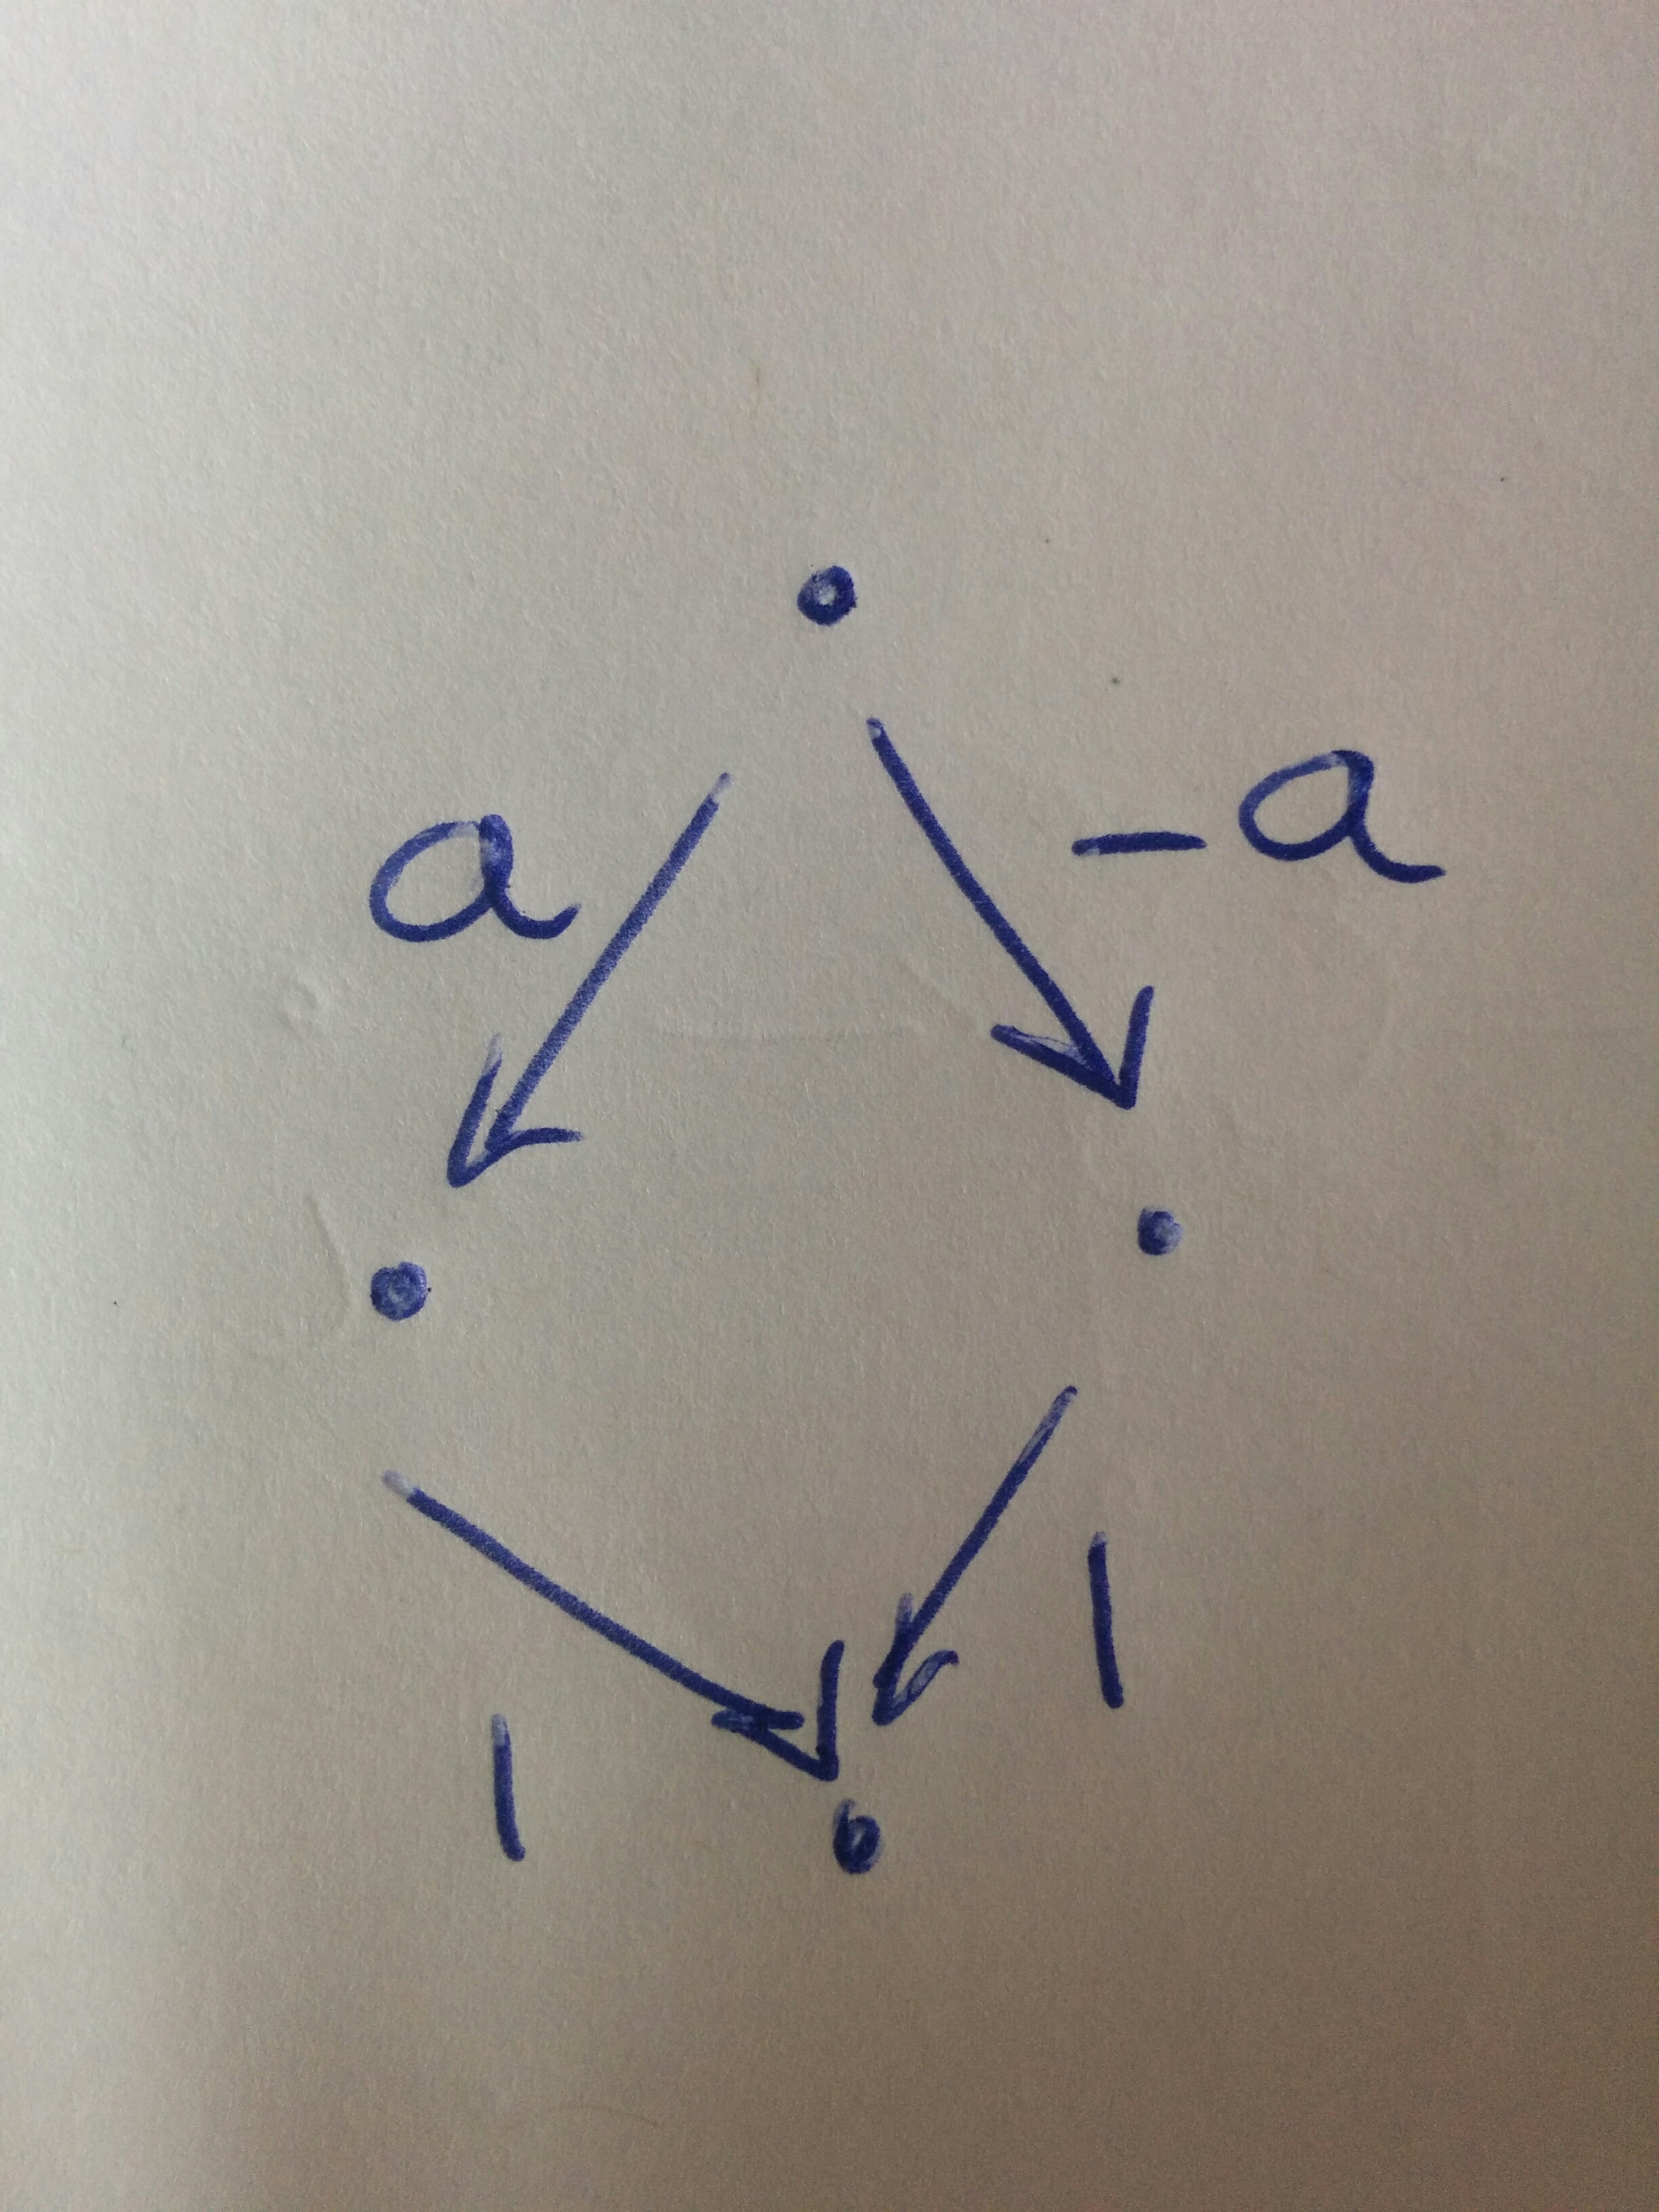
\includegraphics[width=\linewidth]{hand_drawn_example1.jpg}
  \end{subfigure}
  \begin{subfigure}[b]{0.45\textwidth}
    \caption{Graph Corresponding to Example \ref{ex:lag_cancellation}}
    \label{fig:lag_cancellation}
    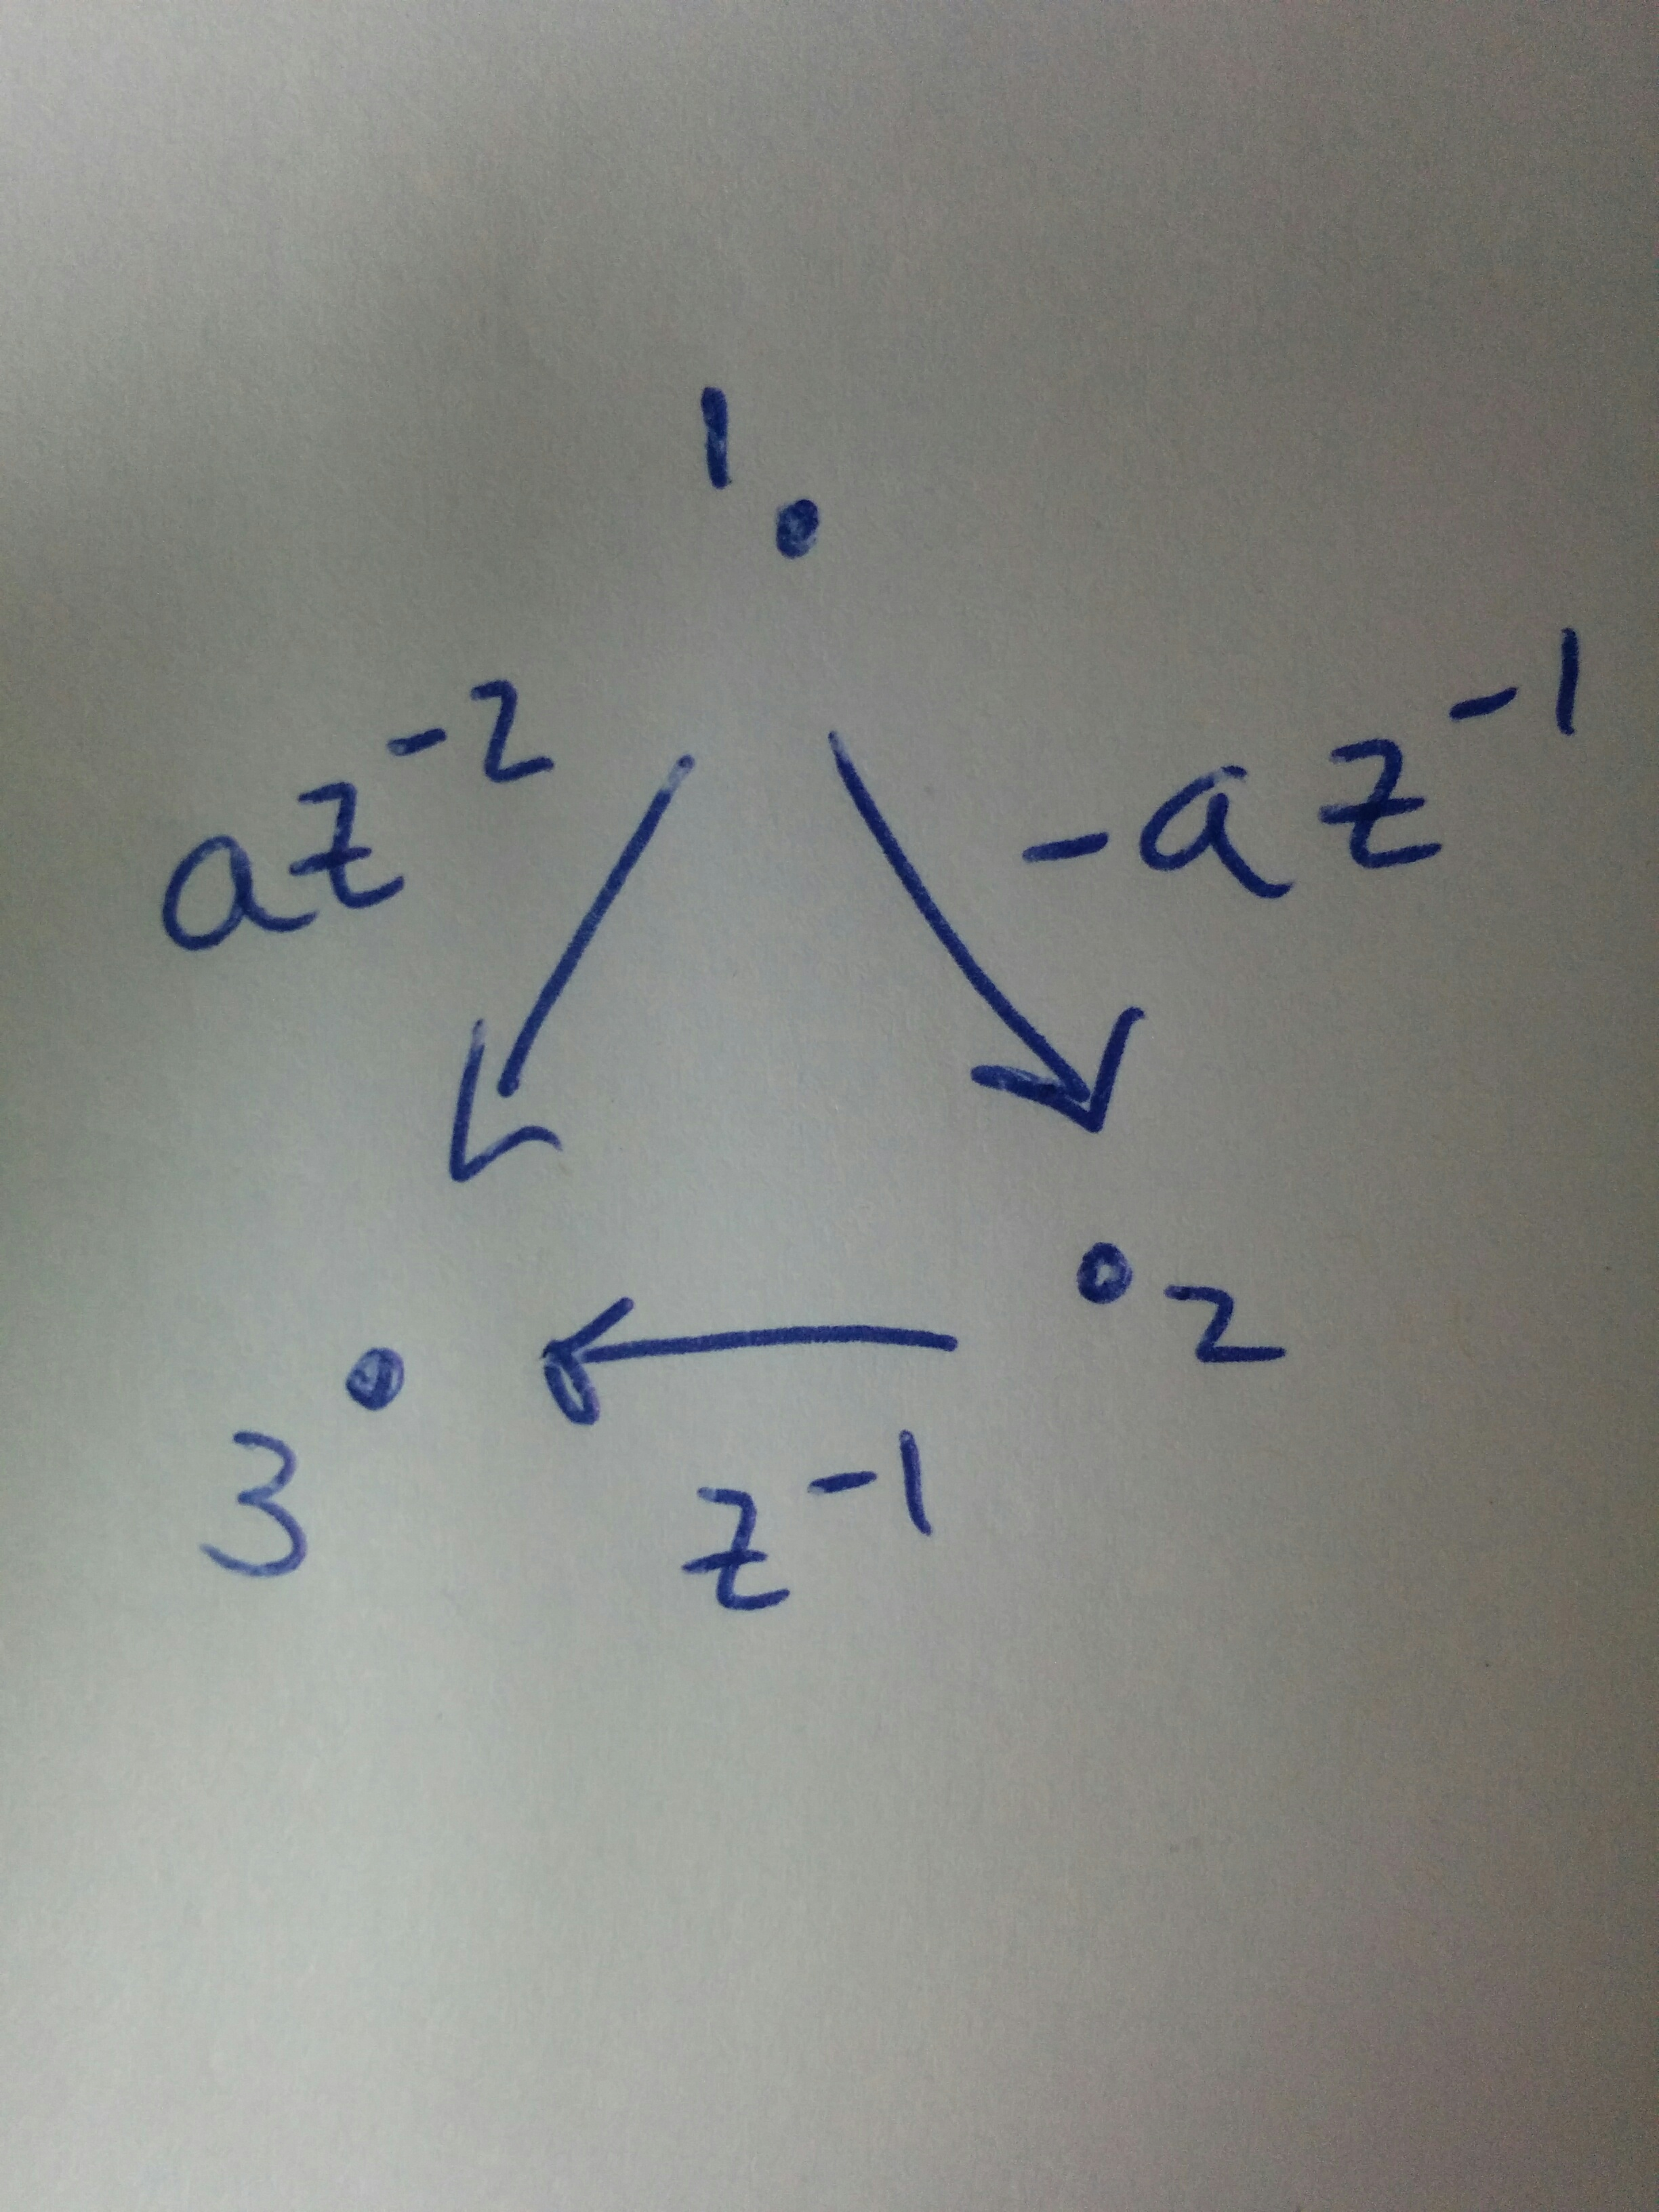
\includegraphics[width=\linewidth]{hand_drawn_example2.jpg}
  \end{subfigure}
\end{figure}

\begin{example}
  \label{ex:lag_cancellation}
  A second example on $n = 3$ nodes is also worth examining, in this case
  cancellation is a result of differing time lags:

\begin{equation*}
  x(t) =
  \left[
    \begin{array}{ccc}
      0 & 0 & 0\\
      -a & 0 & 0\\
      0 & 1 & 0\\
    \end{array}
  \right] x(t - 1) +
  \left[
    \begin{array}{ccc}
      0 & 0 & 0\\
      0 & 0 & 0\\
      a & 0 & 0\\
    \end{array}
  \right] x(t - 2) + v(t)
\end{equation*}

Then

\begin{align*}
  x_2(t) &= v_2(t) - ax_1(t - 1)\\
  x_3(t) &= v_3(t) + x_2(t - 1) + ax_1(t - 2)\\
  \implies x_3(t) &= v_2(t - 1) + v_3(t),
\end{align*}

and again $1 \not\pwgc 3$.
\end{example}

The previous examples seem rather pathological since we have simply
constructed a case where different paths in the graph cancel exactly.
It may be possible to rid ourselves of these pathologies for instance
by defining a notion of ``robust'' pairwise causality where
``$j \pwgc _R i$'' if $j \pwgc i$ almost surely for a ``small'' random
perturbation of the system matrix.  However, we do not believe such a
modification of our theory can have useful practical implications
since the difference between paths that ``nearly cancel'' rather than
cancel exactly would in practice require inordinate amounts of data to
resolve.

Alternatively, we could restrict the coefficients of the system
matrix, e.g. by requiring that $B_{ij}(\tau) \ge 0$.  Instead, we
think it is more meaningful to focus on the defining feature of time
series networks, that is, the topology of $\gcg$.

\begin{definition}[Strongly Causal]
  We will say that a Granger-causality graph $\gcg$ is \textit{strongly causal}
if there is at most 1 directed path between any two nodes.

\hl{TODO: Should DAG be included in this definition?  I think it is
  not necessary for some theorems.}
\end{definition}

Examples of strongly causal graphs include directed trees (or
forests), and DAGs where each node has at most one parent.

\begin{lemma}
  \label{lem:still_strongly_causal}
  If $\gcg$ is a strongly causal graph, any subgraph formed by eliminating nodes
  and all of the in and out edges of the eliminated node is still strongly causal.
\end{lemma}
\begin{proof}
  If $\gcg$ has at most one path between any two nodes, there can only
  be fewer paths after removing nodes from $\gcg$.
\end{proof}


\begin{lemma}
  \label{prop:sc_graph_common_anc}
  In a strongly causal graph if $j \in \anc{i}$ and $k \in \anc{i} \cap \anc{j}$ then the unique path from $k$ to $i$ contains $j$.
\end{lemma}
\begin{proof}
  Suppose that there is a path from $k$ to $i$ which does not contain $j$.  In this case, there are multiple paths from $k$ to $i$ (one of which \textit{does} go through $j$ since $j \in \anc{i}$) which contradicts the assumption of strong causality.
\end{proof}

% Is pwgc transitive?

In light of proposition \ref{prop:sc_graph_common_anc}, the following
provides a converse to proposition \ref{prop:ancestor_properties}.

\begin{proposition}
  \label{lem:pwgc_anc}
  If $\gcg$ is a strongly causal DAG then $j \in \anc{i} \implies j \pwgc i$.
\end{proposition}
\begin{proof}
  Using the representation of equation (\ref{eqn:parent_expansion}) we can represent $x_i(t)$ as

  \begin{equation*}
    x_i(t) = v_i(t) + \B_{ii}(z) x_i(t) + \sum_{k \in \pa{i}}\B_{ik}(z) x_k(t).
  \end{equation*}

  In order to show that $j \pwgc i$ we can show (due to theorem (\ref{thm:granger_causality_equivalences})) that

  \begin{equation*}
    \linE{x_i(t)}{\H_{t - 1}^{(i)}} = \linE{x_i(t)}{\H_{t - 1}^{(i, j)}},
  \end{equation*}

\hl{WIP}

% this allows us to recursively expand the
%   parents of $x_i$ in $\gcg$ in the $\VAR(\infty)$ representation of
%   $x(t)$ since we will eventually terminate at nodes $d$ such that
%   $\pa{d} = \emptyset$.  To this end, examining $x_i$ in equation
%   \ref{eqn:ar_representation}

%   \begin{align*}
%     x_i(t) &= v_i(t) + \sum_{\tau = 1}^\infty \big[ B_{ii}(\tau)x_i(t - \tau) + \sum_{k \in \pa{i}} B_{ik}(\tau)x_k(t - \tau)\big]\\
%     \implies x_i(t) &= (1 - \B_{ii}(z))^{-1} \big[v_i(t) + \sum_{k \in \pa{i}} B_{ik}(\tau)x_k(t - \tau) \big]\\
%     &= \sum_{\tau = 1}^\infty \big[C_{ii}(\tau)v_i(t - \tau) + \sum_{k \in \pa{i}} C_{ik}(\tau)x_k(t - \tau)\big].
%   \end{align*}

%   If $\pa{i} = \emptyset$ then we simply have
%   $x_i(t) = \sum_{\tau = 1}^\infty C_{ii}(\tau)v_i(t)$ and
%   $C_{ii} = A_{ii}$ from equation \ref{eqn:wold}.

%   Applying this relation recursively we can write

%   \begin{equation*}
%     x_i(t) = \sum_{\tau = 1}^\infty\big[C_{ii}(\tau)v_i(t - \tau) + \sum_{k \in \anc{i}}C_{ik}(\tau)v_k(t - \tau) \big].
%   \end{equation*}

\end{proof}

That strong conditions need to be placed on the topology of $\gcg$ in
order for proposition \ref{lem:pwgc_anc} to be true can be seen through the
earlier examples.

\begin{lemma}
  If $\gcg$ is strongly causal, then any $\VAR(p)$ system on $\gcg$ is stable if and only if
  $B_{ii}(z)$ is stable for every $i = 1, \ldots, n$.
\end{lemma}
\begin{proof}
  \hl{This is certainly true, but I don't think I need to use it anywhere.}
\end{proof}

% $B(1) = \left[ \begin{array}{cc} 0 & 1 \\ 1 & 0 \end{array} \right]$

% - - - - - - - - - - - - - - - - - - - - - - - - - - - - - - - - - - - - - - - - - - - - - 
% I'm actually not sure this is true, I think that if there is a common ancestor it is
% ambiguous.  This may be true for transfer entropy, but for Granger-causality even if
% the information arriving at i is later than to j, it may be less corrupt and hence
% still facilitate better predictions about k's future.

% Finally, the \textit{propagation delay} from $j$ to $i$, denoted $d(j, i)$, will be defined as 

% \[
%   d(j, i) = \text{min}\big\{\sum_{k = 0}^{K - 1} d(p_k, p_{k + 1}})\ |\ i = p_0 \rightarrow p_1 \rightarrow \cdots \rightarrow p_K = j \text{ is a path in } \gcg \big\}
% \]

% and $d(j, i) \defeq \text{min}\{B_{i, j}(\tau) \ne 0\}$ if $j \in \pa{i}$.

% - - - - - - - - - - - - - - - - - - - - - - - - - - - - - - - - - - - - - - - - - - - - - 

We are interested in understanding under what conditions a causality
graph can be correctly recovered by pairwise testing alone.  It is not
enough that the graph simply be sparse, as the following example shows.

\begin{example}
  If the causality graph $\gcg$ of the vector process $x(t)$ is
  strongly connected\footnote{there is a directed path from each node
    to every other node}, then the causality graph recovered via
  pairwise causality tests is the complete graph.

  This follows immediately from the fact (lemma \ref{lem:pwgc_anc})
  that $j \in \anc{i} \implies j \pwgc i$.
\end{example}

% \begin{definition}[Simply Causal]
%   If the Granger-Causality graph $\gcg$ for $x(t)$ is as a directed
%   acyclic graph such that there is at most one non-overlapping
%   directed path between any two nodes (excluding self-loops) then we
%   will refer to $\gcg$ as being \textit{simply causal}.
% \end{definition}

% \begin{example}
%   A directed tree (more generally directed forest) is a simply causal
%   graph.
% \end{example}

\begin{lemma}
  If $\gcg$ is a strongly causal DAG then $i \pwgc j$ and $j \in \anc{i}$ are
  \textit{alternatives}, that is $i \pwgc j \implies j \notin \anc{i}$.
\end{lemma}
\begin{proof}
  Suppose that $\gcg$ is a strongly causal DAG and that we have both
  $i \pwgc j$ and $j \in \anc{i}$.  We will show that $i \in \anc{j}$,
  which produces a contradiction (since there must then be a directed cycle).

  Since $j \in \anc{i}$ there is a path $\gcgpath{j}{a}{p}{i}$.
  Moreover, since $i \pwgc j$ by lemma \ref{lem:pwgc_anc} there must
  be a common ancestor $k \in \anc{i} \cap \anc{j}$ (otherwise, we would
  have $i \in \anc{j}$, contradicting the acyclic property).  The node
  $k$ has paths to both $j,\ \gcgpath{k}{b}{q}{j}$ and $i,\ \gcgpath{k}{c}{r}{i}$.

  Now, since the graph is strongly causal, path $c$ must overlap with
  path $a$ from $j$ to $i$ otherwise there would be multiple paths
  from $k$ to $i$.  By the same reasoning with paths from $k$ to $j$,
  the path $c$ must also overlap with path $b$ from $k$ to $j$, so in
  fact path $c$ from $k$ to $i$ is
  $c = b \rightarrow j \rightarrow a$.

  \hl{TODO: We need the strengthening of prop }(\ref{prop:ancestor_properties})\hl{in order to conclude.}

\end{proof}

\subsection{Recovering $\gcg$ via Pairwise Tests}
In this section we will show that if $\gcg$ is a strongly causal DAG, then it is possible to recover $\gcg$ via pairwise tests alone.  This is an interesting fact in and of itself, but also has some implications for applications since pairwise testing is trivially parallelizable.  In section \ref{sec:structure_learning} we will also analyze the use of pairwise testing as a heuristic for general graphs.

\begin{theorem}[Pairwise Recovery]
  \label{thm:tree_recovery}
  If the Granger-Causality graph $\gcg$ for $x(t)$ is a strongly
  causal DAG then $\gcg$ can be inferred from pairwise causality
  tests alone.  The procedure can be carried out, assuming we have an
  oracle for pairwise causality, via algorithm (\ref{alg:pwgr}).

  \begin{algorithm}
    \SetKwInOut{Input}{input}
    \SetKwInOut{Output}{output}
    \SetKwInOut{Initialize}{initialize}
    \DontPrintSemicolon

    \BlankLine
    \caption{Pairwise Graph Recovery}
    \label{alg:pwgr}
    % \TitleOfAlgo{Pairwise Graph Recovery}
    \Input{Pairwise Granger-causality relations between $n$ processes whose joint Granger-causality relations are known to form a strongly causal DAG $\gcg$.}
    \Output{Edges $E = \{(i, j) \in [n] \times [n]\ |\ i \gc j \}$ of the graph $\gcg = ([n], E)$.}
    \Initialize{$S_0 = [n]$  \texttt{\# unprocessed nodes}\\
      $E = \emptyset$  \texttt{\# edges of }$\gcg$\\
      % $P_0 = \emptyset$  \texttt{\# layer by layer driving nodes}\\
      $k = 0$ \texttt{\# a counter used only for notation}}
    \BlankLine
    \While{$S_k \ne \emptyset$}{
      $\widehat{P}_k \leftarrow \{i \in S_{k - 1}\ |\ \forall s \in S_{k - 1}\ s \not\pwgc i\}$  \texttt{\# parents of current layer}\\
      % $P_k \leftarrow P_{k - 1} \cup \widehat{P}_k$ \texttt{\# Expand parent set}\\
      $S_{k + 1} \leftarrow S_k \setminus \widehat{P}_k$ \texttt{\# remove from } $S$\\

      \;
      $C_k \leftarrow \{i \in S_{k + 1}\ |\ \forall s \in S_{k + 1}\ s \not\pwgc i\}$   \texttt{\# potential children of }$P_k$\\

      \For{$r = 0, \ldots, k$}
      {
        $D_{kr} \leftarrow \{(i, j) \in \widehat{P}_{k - r} \times C_k\ |\ i \pwgc j,\ \text{no } i \rightarrow j \text{ path in } E \}$\\%  \texttt{\# edges incident on }$C_k$\\
        $E \leftarrow E \cup D_{kr}$ \texttt{\# add edges to }$E$\\
      }

      \;
      $k \leftarrow k + 1$
    }
    \Return{$E$}
  \end{algorithm}
\end{theorem}

We prove the theorem by establishing the correctness of algorithm (\ref{alg:pwgr}).  The idea is to iteratively ``peel away layers'' of nodes by removing the nodes that have no parents remaining, which always exist since the graph is acyclic.  The additional requirement of strong causality ensures firstly that all actual edges of $\gcg$ manifest in some way as pairwise relations (by proposition \ref{prop:pwgc_anc}), and secondly, as we will see, that parents of $C_k$ are in $\bigcup_{r = 0}^k\widehat{P}_{k - r}$ and can be determined by a pairwise test.

\begin{example}
  That we need to proceed backwards through $\widehat{P}_{k - r}$ can be seen from the example of figure \ref{fig:example_fig3}, where if $D_k = \{(i, j) \in \Big(\bigcup_{r = 0}^k \widehat{P}_{k - r}\Big) \times C_k\ |\ i \pwgc j \}$ above we would infer the false positive edge $2 \rightarrow 3$.  Moreover, the same example shows that if simply $D_k = \{(i, j) \in \widehat{P}_k \times C_k\ |\ i \pwgc j \}$, then the edge $1 \rightarrow 3$ would be missed.

\hl{TODO: Inkscape figure}

  \begin{figure}
    \centering
    \label{fig:example_fig3}
    \caption{Example graph for Algorithm \ref{alg:pwgr}}
    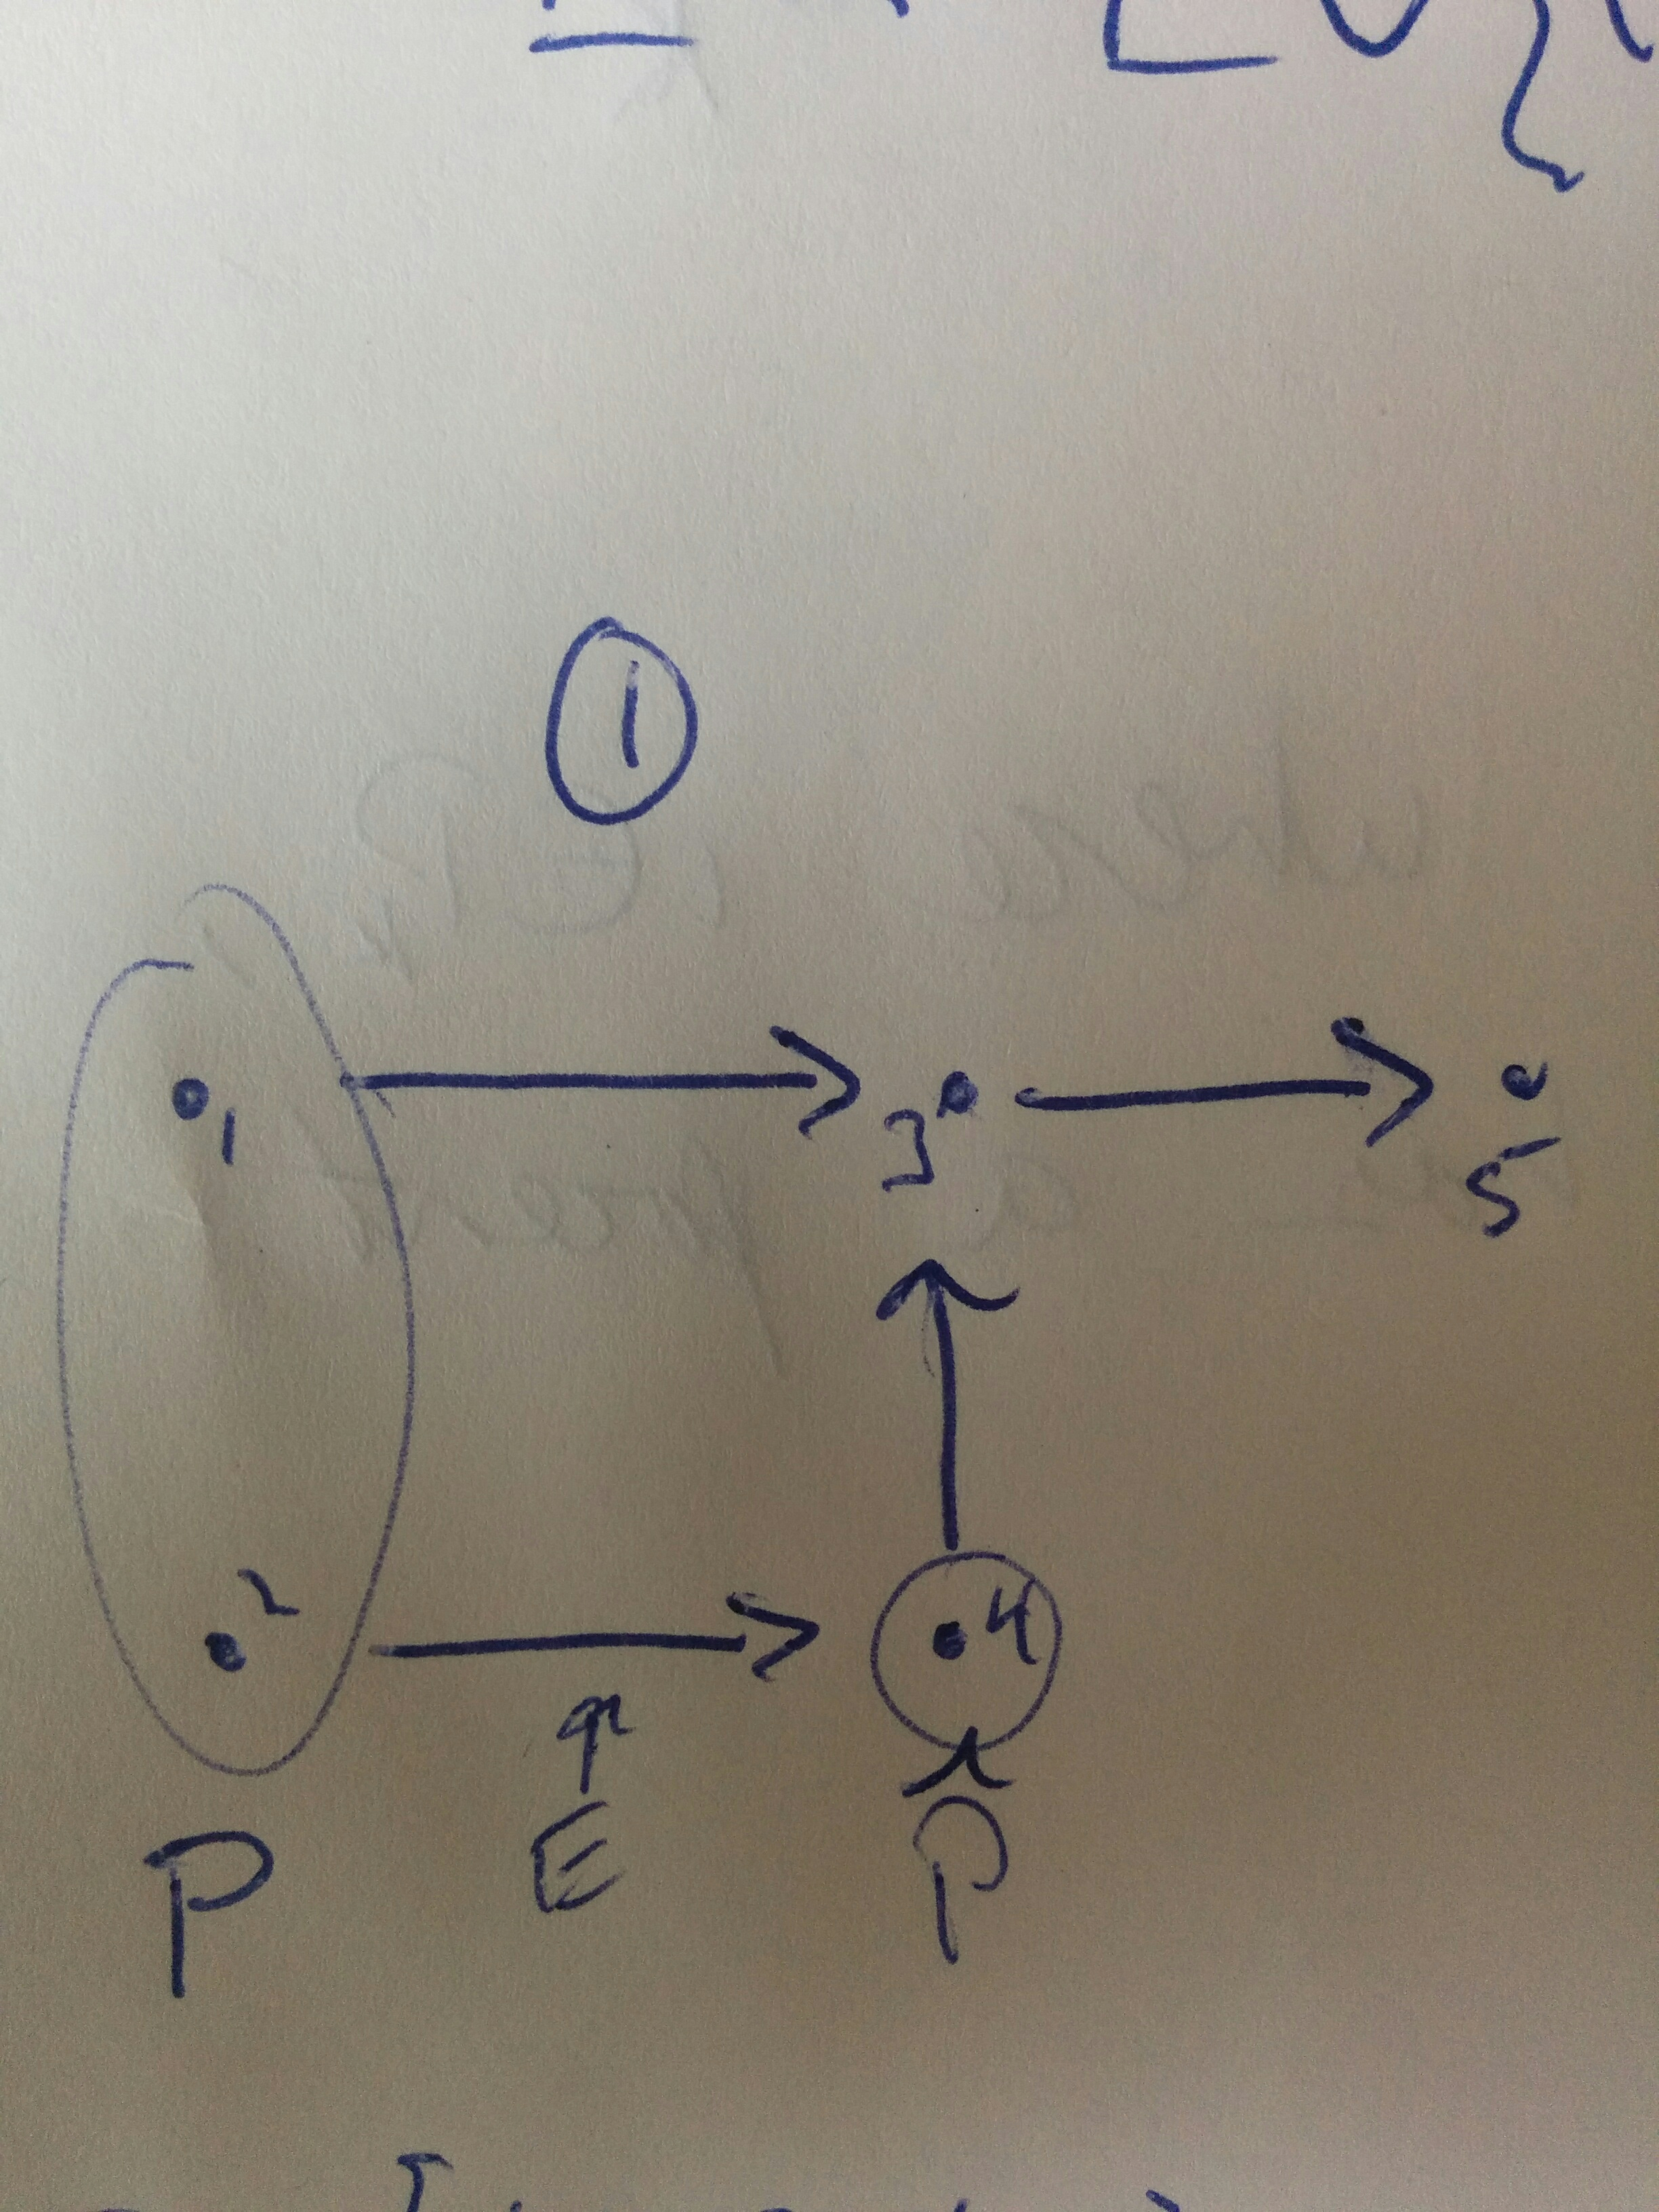
\includegraphics[width=0.5\linewidth]{hand_drawn_example3.jpg}
  \end{figure}
\end{example}

\begin{proof}
% 1. Dispense with trivialities
% 2. Show that hat{P}_k is nonempty
% 3. Show that C_k is nonempty
% 4. Show that edges in D_k are actual edges in G
% 5. show that each edge incident on C_k is in D_k
% 6. Induction

  Firstly, if $n = 0$ or $n = 1$ the algorithm is trivially correct, returning on the first iteration with $E = \emptyset$.  Suppose then that $n > 1$, we will proceed by induction.

On the first iteration of the algorithm ($k = 0$) we have $S_0 = [n]$ and $E = \emptyset$.  The set $\widehat{P}_0$ is non-empty since $\gcg$ is a DAG and therefore there are nodes in $\gcg$ without parents, thence if $\widehat{P}_0 = \emptyset$ proposition \ref{prop:ancestor_properties} would be contradicted.  Now, if $\widehat{P}_0 = [n]$ then the graph necessarily contains no edges and we will correctly return $E = \emptyset$.  On the other hand, if $\widehat{P}_0 \ne [n]$ then $C_0$ must also be non-empty, otherwise there would be driving nodes not included in $\widehat{P}_0$.  Consider now an edge $(i, j) \in D_0$ ($D_0$ is non-empty for the same reason as $C_0$).  Since $i$ has no parents, $\anc{i} \cap \anc{j} = \emptyset$ and therefore $i \in \anc{j}$ (proposition \ref{prop:ancestor_properties}).  Furthermore, the construction of $C_k$ implies that $i \in \pa{j}$ since otherwise, there would be some $u \in \anc{j}$ with $i \in \anc{u}$, but then by proposition \ref{lem:pwgc_anc} $i \pwgc u$ and $u \pwgc j$ so that $u \not \in \widehat{P}_0 \implies u \in S_0 \implies j \not\in C_0$, a contradiction.

% and show that on each step, every edge incident upon a node in $C_k$ is contained in $D_k$, that every edge in $D_k$ is an edge in $\gcg$, and finally that $\bigcup_{k = 1}^n C_k = [n] \setminus \widehat{P}_0$ and that this implies $\big([n], \bigcup_{k = 1}^n D_k\big) = \gcg$.


%  On the first iteration of the algorithm ($k = 0$) we have $S_0 = [n]$ and $E_0 = \emptyset$.  The set $\widehat{P}_0$ is non-empty since $\gcg$ is a DAG and therefore there are nodes in $\gcg$ without parents, thence if $\widehat{P}_0 = \emptyset$ proposition \ref{prop:ancestor_properties} would be contradicted.  Now, if $\widehat{P}_0 = [n]$ then the graph necessarily contains no edges and we will correctly return $E = \emptyset$.  On the other hand, if $\widehat{P}_0 \ne [n]$ then $C_0$ must also be non-empty, otherwise there would be driving nodes not included in $\widehat{P}_0$.  Consider now an edge $(i, j) \in D_0$ (again $D_0$ is non-empty for the same reason as $C_0$).  Since $i$ has no parents, we must have $\anc{i}\cap\anc{j} = \emptyset$ and therefore $i \in \anc{j}$, and due to the construction of $C_0$ we in fact have $i \in \pa{j}$, which establishes that every edge in $D_0$ is also an edge in $\gcg$.  Finally consider $j \in C_0$, by proposition \ref{prop:pwgc_anc} and since the parents of $C_0$ must be in $P_0$, we see that every edge incident on $j$ must be present in $D_0$.

% We also see that since nodes in $\widehat{P}_0$ have no parents,

% we must have $\anc{i}\cap\anc{j} = \emptyset$, and therefore by proposition \ref{prop:ancestor_properties} $i \in \anc{j}$;  moreover, the construction of $\widehat{P}_1$ implies that in fact $i \in \pa{j}$, so $(i, j)$ is an edge of $\gcg$.

%Finally, by similar reasoning, there cannot be an edge $(i, j) \in D_0$ which is not in $\gcg$, since $\anc{i} \cap \anc{j} = \emptyset$.

%Consider now step $K < n$ of algorithm \ref{alg:pwgr}.  By lemma \ref{lem:still_strongly_causal} the graph remains strongly causal after having removed nodes $\bigcup_{k = 0}^K P_k$ from $S$, and we assume for induction that $\bigcup_{k = 1}^K D_k$ are all edges of $\gcg$.

\hl{WIP}
\end{proof}

\begin{example}
  Being a strongly causal DAG is merely a sufficient condition.  For example, the complete directed graph with 2 nodes (e.g. $B(1) = \left[ \begin{array}{cc} 1/2 & 1 \\ 1 & 1/2 \end{array} \right]$) contains a loop but is pairwise recoverable, though not by algorithm (\ref{alg:pwgr}).  Clearly, this example is somewhat artificial since when $n = 2$ there is no difference between pairwise Granger-causality and joint Granger-causality amongst all series -- however, one can take any strongly causal DAG, and then add two additional nodes having such a loop without impacting the pairwise recoverability.
\end{example}

\section{Structure Learning}
\label{sec:structure_learning}
\subsection{Local Search Heuristics}


\subsection{Edge-Wise Grouped LASSO}
Minimize the sparsity promoting regularized least squares problem and choose the hyper-parameters against the Akaike information criteria.

\begin{equation}
  L(\lambda, p) \defeq \underset{B}{\text{minimize}}\ \frac{1}{T}\sum_{t = 1}^T||x(t) - \sum_{\tau = 1}^pB(\tau)x(t - \tau)||_2^2 + \lambda \sum_{i, j}\big[\alpha||B_{i, j}||_2 + (1 - \alpha)||B_{i, j}||_1\big]
\end{equation}

\begin{equation}
  \underset{\lambda, p}{\text{minimize}}\ L(\lambda, p) + \mathsf{AIC}(B^{(\lambda, p)})
\end{equation}

\subsection{Bayesian Posterior Thresholding}
Consider the Bayesian model

\begin{equation}
  \begin{aligned}
    (x(t)\ |\ B, \sigma_v^2, \{x(t - \tau)\}_{\tau = 1}^p) &\sim \mathcal{N}(\sum_{\tau = 1}^pB(\tau)x(t - \tau), \sigma_v^2)\\
    (B_{ij}(\tau)\ |\ G_{ij}(\tau)) &\sim G_{ij}(\tau)\mathcal{N}(0, \sigma_\beta^2) + (1 - G_{ij}(\tau))\delta_0(B_{ij}(\tau))\\
    (G_{ij}(\tau)) &\sim \mathsf{BER}(p_{ij}(\tau))\\
    \sigma_v^2 &\sim \Gamma(a_v, b_v)\\
    \sigma_\beta^2 &\sim \Gamma(a_\beta, b_\beta)
  \end{aligned}
\end{equation}

Similar models have been studied by various authors in the context of the linear regression model \hl{[(cite them)]} where it is referred to as \textit{stochastic variable selection}, or referred to as a model for Bayesian variable selection.

Since we have in mind applications where $n$ is large, sampling posterior probabilities can be prohibitively burdensome, so we can instead fit the mean-field variational approximation $p(B, G, \sigma\ |\ X) \approx q_Gq_Bq_\sigma$ and subsequently apply a thresholding operation to the posterior edge inclusion probabilities under $q_G$.

\subsection{Pairwise Minimum Error Spanning Trees}
Inspired by theorem \ref{thm:tree_recovery}, we propose the following
structure learning heuristic.

%% This algorithm should perform coordinate descent or jointly refit all the trees.

\begin{enumerate}
  \item{Set $k = 0$ and $x^0(t) = x(t)$}
  \item{Compute all pairwise causality measures $\Xi \defeq \big[\ln \frac{\xi_i}{\xi_{ij}} \big]_{i, j}$}
  \item{Find the maximum spanning arborescence\footnote{An ``arborescence'' is a french word for a tree diagram, and refers to a \textit{directed} tree in graph theory} $\mathcal{T}_k$ of a graph having edge weights $\Xi_{ij}$.}
  \item{Fit a vector LTI filter $F_k$ having graph defined by $\mathcal{T}_k$ to $x^{k - 1}(t)$ and set $x^k(t) = x^{k - 1}(t) - \hat{x}^{k - 1}(t)$}
  \item{Repeat over $k$ until a stopping criteria is met}
\end{enumerate}


\section{Application}
\section{Conclusion}

\printbibliography
\end{document}

%%% Local Variables:
%%% mode: latex
%%% TeX-master: t
%%% End:
